\subsection{Analog-To-Digital Converter:}

The circuit presented in Figures 4.0 and 4.1 it's the same that we have analyzed in {\itshape section's 3} Figure 3.0.

\begin{figure}[H]
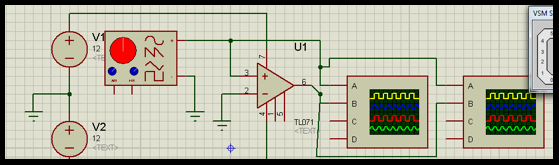
\includegraphics[height = 9cm, width = 16.5cm]{s1.png}
\centering \linebreak \linebreak {\small Figure 4.0: Analog-to-digital converter simulated circuit with a Sensor-Voltage $V_{a}$ = 0.42 V.}
\end{figure}

\begin{figure}[H]
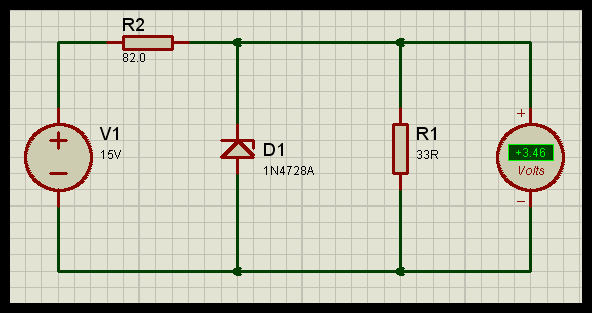
\includegraphics[height = 9cm, width = 16.5cm]{s2.png}
\centering \linebreak \linebreak {\small Figure 4.1: Analog-to-digital converter simulated circuit with a Sensor-Voltage $V_{a}$ = 0.27 V.}
\end{figure}

\pagebreak

Same as section 3, we capture the results in Table 2 according to the development's Table's 1 column {\bfseries sensor voltage} to see if the simulated values are similar. Figure 4.0 represents the higher input voltage measured and Figure 4.1 the lowest input voltage. As we can see the simulated values are exactly the same as the development ones. \hfill \break

\begin{center}
\begin{tabular}{c c c c}
\toprule \toprule
\hspace{40px} Sensor Voltage \hspace{40px} & \hspace{30px} Temperature \hspace{30px} & \hspace{30px} Binary Combination \hspace{30px} \\
\midrule \midrule
0.42 V & $42^{\circ}$ & 0010 1011 & \\
\midrule
0.39 V & $39^{\circ}$ & 0010 1000 & \\
\midrule
0.36 V & $36^{\circ}$ & 0010 0101 & \\
\midrule
0.35 V & $35^{\circ}$ & 0010 0100 & \\
\midrule
0.33 V & $33^{\circ}$ & 0010 0010 & \\
\midrule
0.31 V & $31^{\circ}$ & 0010 0000 & \\
\midrule
0.29 V & $29^{\circ}$ & 0001 1110 & \\
\midrule
0.27 V & $27^{\circ}$ & 0001 1100 & \\
\bottomrule
\end{tabular}
\centering \linebreak \linebreak Table 2: Simulated results.
\end{center}

\pagebreak